\documentclass[
        a4paper,     % Format A4
        titlepage,   % mit Titelseite
        twoside,     % zweiseitig
        parskip      % mit Durchschuss
                                 % (= Abstand zwischen Absätzen, statt Einrückung)
        ]{scrartcl} %{} % KOMA-Script Grundklasse     texdoc scrguide

\usepackage[american]{babel}             
\usepackage[T1]{fontenc}          % Schriftkodierung mit Umlauten
\usepackage{textcomp,amsmath}     % Mathezeichen etc.
\usepackage{graphicx}             % Graphiken einbinden


\usepackage{acro}                 % List of abbriviations 
\usepackage[toc,page]{appendix}   % Appendixes
\usepackage{listings}             % Code Blocks
\usepackage{color}

\usepackage{microtype} 			  % enable margin kerning
\usepackage{tabularx}		      % table stuff
\usepackage{booktabs}			  % table stuff, like toprule
\usepackage{todonotes}
\usepackage{colortbl}
\usepackage{tipa}
\usepackage{amsfonts}

% Table styles % 
\setlength{\tabcolsep}{18pt}
\renewcommand{\arraystretch}{1.5}

\definecolor{lightgray}{rgb}{0.9, 0.9,0.9}

% Code Listing Styles
\definecolor{backcolour}{rgb}{0.95,0.95,0.92}
\lstdefinestyle{mystyle}{
    backgroundcolor=\color{backcolour},   
    captionpos=b,
    breaklines=true,
    basicstyle=\footnotesize,
    numbers=left,                    
    numbersep=5pt,  
}
\lstset{style=mystyle}

% probably a good idea for the nomenclature entries:
\acsetup{first-style=short}

% bibtex
\usepackage{url}
\bibliographystyle{ieeetr}      

\titlehead{

\includegraphics{hpi_logo_cmyk_wb_sl2}
} \subject{Master's Thesis}
\title{Language Identification Using Deep Convolutional Recurrent Neural Networks
\\ \bigskip 
\large{<Deutscher Titel bei englischer Arbeit> }}
\author{Tom Herold\\{\small{\url{tom.herold@student.hpi.uni-potsdam.de}}}}
\date{XX.0X.2017}
\publishers{
Supervisors \\ Prof. Dr. Christoph Meinel \\ Dr. Haojin Yang \\
\bigskip
Internet Technologies and Systems \\
Hasso Plattner Institute \\
University of Potsdam, Germany
}

\frenchspacing
\usepackage{siunitx}

\newcommand{\matsym}[1]{\boldsymbol{#1}}
\newcommand{\vecsym}[1]{\boldsymbol{#1}}

\pagestyle{headings}    % Seitenstil mit Kapitelüberschriften in der Kopfzeile

% class `abbrev': abbreviations:
\DeclareAcronym{ann}{
  short = ANN,
  long = artificial neural network,
  class = abbrev
}
\DeclareAcronym{dnn}{
  short = DNN,
  long = deep neural network,
  class = abbrev
}
\DeclareAcronym{rnn}{
  short = RNN,
  long = recurrent neural network,
  class = abbrev
}
\DeclareAcronym{cnn}{
  short = CNN,
  long = convolutional neural network,
  class = abbrev
}
\DeclareAcronym{crnn}{
  short = CRNN,
  long = convolutional recurrent neural network,
  class = abbrev
}
\DeclareAcronym{lstm}{
  short = LSTM,
  long = long short-term memory,
  class = abbrev
}
\DeclareAcronym{eer}{
  short = EER,
  long = equal error rate,
  class = abbrev
}
\DeclareAcronym{far}{
  short = FAR,
  long = false accept rate,
  class = abbrev
}
\DeclareAcronym{fc}{
  short = FC,
  long = fully connected layer,
  class = abbrev
}
\DeclareAcronym{frr}{
  short = FRR,
  long = false reject rate,
  class = abbrev
}
\DeclareAcronym{gpu}{
  short = GPU,
  long = graphics processing unit,
  class = abbrev
}
\DeclareAcronym{mlp}{
  short = MLP,
  long = multilayer perceptron,
  class = abbrev
}
\DeclareAcronym{mse}{
  short = MSE,
  long = mean squared error,
  class = abbrev
}
\DeclareAcronym{nist}{
  short = NIST,
  long = National Institute of Standards and Technology,
  class = abbrev
}
\DeclareAcronym{pca}{
  short = PCA,
  long = principal component analysis,
  class = abbrev
}
\DeclareAcronym{pdf}{
  short = PDF,
  long = probability density function,
  class = abbrev
}
\DeclareAcronym{relu}{
  short = ReLU,
  long = Rectified Linear Unit,
  class = abbrev
}
\DeclareAcronym{roc}{
  short = ROC,
  long = receiver operating characteristic,
  class = abbrev
}
\DeclareAcronym{sgd}{
  short = SGD,
  long = stochastic gradient descent,
  class = abbrev
}
\DeclareAcronym{svm}{
  short = SVM,
  long = support vector machine,
  class = abbrev
}
\DeclareAcronym{tar}{
  short = TAR,
  long = true accept rate,
  class = abbrev
}
\DeclareAcronym{lid}{
  short = LID,
  long = language identification,
  class = abbrev
}
\DeclareAcronym{tsne}{
  short = t-SNE,
  long = t-distributed stochastic neighbor embedding,
  class = abbrev
}



\begin{document}

    \pagenumbering{roman}
    \maketitle    %  Titelseite erzeugen

    \cleardoublepage % neue Doppelseite


    \section*{\LARGE Abstract}
With the increasing ubiquity of voice input systems to computers users rely on robust speech recognition algorithms to process these intents. The first step and key component to automatic speech recognition is language detection. Without automatic language detection all subsequent recognition steps will fail because they can neither parse the speech utterances correctly nor apply proper grammar.

A second trend in computer science is the successful application of deep neural networks on a variety of problems. In this thesis, we present a hybrid neural network system using deep learning techniques for automatic language identification for speech audio samples. Specifically, we apply convolutional recurrent neural networks on human speech inputs and evaluate their robustness in different environments.

Convolutional neural networks have shown great promise within the computer vision research community. Therefore, we base our research on established model architectures such as the Inception network\cite{szegedy2015going} and transfer our audio-based research task into the image processing domain. We study the effectiveness of spectrogram images as a valuable input feature. We discuss additional audio representations and related work for speech processing systems.

Deep learning systems benefit greatly from the availability of large-scale datasets. We train our models on more than \num{1000} hours of speech audio in six different languages: English, German, French, Spanish, Mandarin Chinese and Russian. We collect and process this data from speeches and session from the European Parliament as well as from news channels such as the BBC hosted on YouTube.

Our best performing convolutional recurrent neural network scores a top accuracy and F1 score of \SI{96}{\percent} on the news dataset. With this approach, we report a constant improvement over various baseline convolutional neural networks. We evaluate our models in diverse noisy scenarios with data augmented to include white noise, crackling noise, and background music and observe a decrease in accuracy by 5 percentage points (p.p.), 3 p.p., 7 p.p, respectively. On the smaller EU dataset we achieve an accuracy and F1 score of~\SI{98}{\percent}.

    \cleardoublepage
    \section*{\LARGE Zusammenfassung}
Computern mit Spracheingabem\"oglichkeiten sind immer h\"aufiger anzutreffen. Deshalb sind Nutzer vermehrt auf verl\"assliche Spracherkennungsalgorithmen angewiesen. Dabei ist automatische Sprachidentifizierung der erste und wichtigste Schritt f\"ur die eigentliche Spracherkennung. Ohne automatische Sprachidentifizierung sind alle weiteren Erkennungsschritt nutzlos, da weder Sprachkl\"ange richtig verarbeitet noch Grammatikregeln ordentlich angewandt werden.

Ein zweiter aktueller Trend in der Informatik ist die erfolgreiche Anwendung von tiefen neuronalen Netzwerken f\"ur eine Vielzahl von Aufgabenstellungen. In dieser Arbeit wird ein hybrides, neuronales Netzwerkmodell zur automatischen Identifizierung unterschiedlicher Sprachen mithilfe von \emph{deep learning} Techniken vorgestellt. Im Speziellen werden mehrere \emph{convolutional recurrent neural network} Modelle auf menschliche Spracheingaben angewandt und deren Robustheit in verschiedenen Ger\"auschumgebungen evaluiert.

\emph{Convolutional neural networks} haben innerhalb der automatischen Bilderkennungsforschung beachtliche Durchbr\"uche erzielt. Deshalb wird unsere audiobasierte Forschungsfrage in die Bildverarbeitungsdom\"ane eingebettet. Dar\"uber hinaus basiert diese Arbeit auf deren etablierten Modellarchitekturen, wie beispielsweise das Inception Netzwerk\cite{szegedy2015going}. Dabei wird die Effektivit\"at von Spektrogrammbildern als zielf\"uhrendes Eingabemedium analysiert. Zus\"atzlich werden weitere Audiorepr\"asentationen und weiterf\"uhrende Publikationen vorgestellt.

Insbesondere die Verf\"ugbarkeit von gro{\ss}en Datens\"atzen kommen \emph{deep learning} Systemen zu Gute. Unsere Modelle werden auf mehr als \num{1000} Stunden an Sprachaufnahmen in sechs verschiedenen Sprachen trainiert: Englisch, Deutsch, Franz\"osisch, Spanisch, Mandarin und Russisch. Die Datengrundlage bilden Reden und Sitzungen des Europ\"aischen Parlaments, sowie YouTube Kan\"ale verschiedener Nachrichtensender, wie beispielsweise der BBC.

Unser leistungsf\"ahigstes \emph{convolutional recurrent neural network} Modell erreicht eine Erkennungsgenauigkeit und ein F-Ma{\ss} von \SI{96}{\percent} auf dem Nachrichtendatensatz. Unser Ansatz stellt eine konstante Verbesserung gegen\"uber allen getesteten \emph{convolutional neural networks} dar. Die Modelle werden zus\"atzlich in verschiedenen Szenarien mit k\"unstlich ver\"anderten Daten evaluiert: Dabei f\"ugen wir St\"orger\"ausche, wie Rauschen, Geknister und Hintergrundmusik zu den Daten hinzu und messen einen Genauigkeitsverlust von jeweils 5 Prozentpunkten (PP), 3 PP und 7 PP gegen\"uber den Originaldaten. Auf dem kleineren EU-Datensatz erreichen wir eine Genauigkeit und ein F-Ma{\ss} von \SI{98}{\percent}.
    \cleardoublepage
    \section*{\LARGE Acknowledgments}
I would like to express my gratitude to my supervisors Dr. Haojin Yang and Prof. Dr. Christoph Meinel. I want to thank them for giving me the opportunity to research this interesting topic, as well as for their guidance and advice. I especially want to thank Dr. Yang for his insights, support, and inspiration regarding the deep learning techniques used in my master's thesis.

I would also like to thank my colleagues Georg Wiese, Christian Bartz, Tom Bocklich, Norman Rzepka, Christoph Sterz, and Johannes Jasper for the many fruitful discussions about language identification and machine learning in general. I owe them a great deal of gratitude for supporting and encouraging me while working on this thesis. I am also very grateful for the stylistic critique, review, and language support by Christoph Sterz and Patrick L\"uhne.

Thank you.


    \cleardoublepage
    
    \tableofcontents
    \clearpage
    \printacronyms[include-classes=abbrev,name=Abbreviations]

    \pagenumbering{arabic}
    \section{Introduction}

\subsection{Language Identification as the key to speech tasks}


Current generation language system are already available and in production for a number of industries. To make customer support more helpful and user friendly some call centers apply language identification systems to route customers to native speaking

Law enforcement agency deploy language identification systems for identifying suspect locations based on speech features and accents in telephony data. \todo{Source}. To foster research in this field DARPA established the TIMIT dataset for language identification of North American speakers. \todo{source}

At the time of this writing we had to acknowledge that not even Google Translate has automated language detection to determine the input language for a speech sample. Automated input language detection is available for written texts but Google Translate's voice input feature is only available for use after manually selection an input language. We believe that having an automated language detection system could be extremely helpful to users. 

Not only would this improve mobile and hands free interaction with the tool but also bring us closer to a



\subsection{Contributions}
In this thesis we present an approach to language identification systems. We approach this task by using deep learning techniques. We transfer the given audio classification problem into an image based task to apply image recognition algorithms. Our contributions can be summarized as follows:
\begin{itemize}
	\item We investigate the suitability of convolutional neural networks to the task of language identification. We propose a hybrid network, combing the descriptive powers of convolutional neural networks with the ability of recurrent neural networks to learn time series. This approach is called convolutional recurrent neural network (CRNN). 
	\item We implemented a Python system of such a CRNN approach using the deep learning framework Keras and TensorFlow. 
	\item In train our system we gather our own large scale dataset of audio recordings. We explain how we obtained more than a thousand hours of human speech data suitable for our task.
	\item We assessed several machine learning metrics on our system with respect to our test data. Furthermore, we investigated the influence of noisy environments on our system. We discuss the system's ability to differentiate between several languages and how such a system can be extended to more languages.
	\item To showcase our system we developed a web service demo application using our best performing model. Further, we published said model for use by others.
\end{itemize} 


\subsection{Outline of the Thesis}
This thesis is structure as follows: In chapter \ref{sec:lid} we introduce the language identification problem and state our research hypotheses. Chapter \ref{sec:theoretical_background} explains the theoretical background of the deep learning techniques used in this thesis. In chapter \ref{sec:results_eu}} , we will 

    \section{The Language Identification Problem}
\label{sec:lid}

\subsection{Language Identification as the key to speech tasks}

Automatic language identification (\ac{lid}) is the process of determining the language spoken in an audio recording. The language identification systems proposed in this thesis consume audio recordings and use deep learning techniques to do an automated classification of the recording's source language.
Language identification is often the first step in a natural language processing pipelines. Automatic language identification systems can serve a wide variety of applications from industry and research to entertainment. 

In contrast to LID systems, automatic speech recognition (\ac{asr}) is the task of transcribing spoken language into readable text, sometimes also known as speech-to-text system. Selecting the correct input language for these systems is crucial for transcribing single letters into meaningful words and correct grammar. Many commercially available ASR system require manual setting of the input language and would benefit greatly from an automated language identification system as part of their processing pipeline.

Many call center operators benefit from LID systems by automatically routing telephone calls to connect a caller with a suitable native speaker. This approach can be used both for customer care hotlines connecting callers with help desk agents as well governments agencies such as emergency telephone services. Muthusamy et al. report that manual matching emergency calls to US law enforcement agencies with native speaking agents can involve a significant delay of up to three minutes. Automatic language identification systems could speed up this process and efficiently support human agents~\cite{muthusamy1994reviewing}.

Similarly to language identification some research is focused on dialect detection. To foster research in this field, DARPA established the TIMIT dataset for dialect identification of North American speakers~\cite{garofolo1993darpa}. The dataset features eight major North American dialects and has long been the default corpus for comparative research on lid systems.
Recently, Germany's Federal Office for Migration and Refugees (BAMF) announced the plans for using dialect identification systems\footnote{\url{http://www.theverge.com/2017/3/17/14956532/germany-refugee-voice-analysis-dialect-speech-software, accessed 13.04.2017}} as an additional resource in identifying a person's origin.

Language identification is also the first step to translation tasks. At the time of this writing we discovered that not even the Google Translate mobile app has automated language detection to determine the input language for a speech sample. Automated input language detection is available for written texts but Google Translate's voice input feature is only available for use after manually selecting an input language. We believe that having an automated language detection system could be extremely helpful to users. 

An ever increasing number of people connect to the internet or communicate with each other using their smartphone. While touchscreen input can be complicated in some situations, the demand for voice interactions grows steadily. Many tasks can already be solved through voice input. This hands free, voice enabled interaction is trend that we see in other industries such as automative computing as well.

Automatic LID systems and machine intelligence are also helpful for some entertainment companies. When we first started working on this thesis we were briefly inspired by the challenges of Berlin based startup Dubsmash\footnote{\url{https://www.dubsmash.com/}, accessed 13.04.2017}. Their app lets user's create a mashup of a large variety of existing songs, movie quotes, or other voice snippets with a ten-second video recording of the user. The resulting video clip can be shared with friends and usually features a funny and personal reinterpretation of the audio source's original context. The success of the app is directly proportional to user's interest in the offered sound clips. In some cases, however, users were offered clips in foreign languages which were often perceived as not funny or inappropriate. In this case, a LID system could be used to classify the language of the millions of audio snippets available in their library. Consequently, only sounds in the user's native language can be recommended to the user.


\subsection{Task Specification in This Thesis}
In this thesis we propose a language identification (\ac{lid}) system for classifying the languages of a given audio recording. Our system is trained using human voices recordings. We evaluate the suitability of convolutional neural networks for a LID system. Finally, this approach is extended with a recurrent neural network to compose a hybrid network known as convolutional recurrent neural network (\ac{crnn}). The system 's performance is evaluated on a set of news broadcasts and speeches made by members of the European Parliament. We further assess the system's robustness to noisy environments and background music. This thesis states the following hypotheses:

\begin{enumerate}
	\item Convolutional neural networks can be successfully used for language identification tasks with high accuracy.
	\item Spectrogram images are a suitable input representation for learning audio features.
	\item Convolutional recurrent neural networks improve the classification accuracy for our LID task compared to a CNN based approach.
\end{enumerate}



    \section{Theoretical Background}
\label{sec:theoretical_background}
In this chapter we introduce the theoretical background of the machine learning algorithms used throughout this thesis. We explain the different machine learning concepts and the purpose of a classifier. Furthermore, we lay the foundations for the individual build blocks and layers of deep neural network system. We explain the differences between convolutional neural network and recurrent neural networks and follow up by describing hybrid models constructed of both of these. More specifically, we describe the convolutional recurrent neural network (CRNN) architecture as used in this thesis. Finally, we present different representations for audio file suitable for machine learning tasks.

\subsection{Machine Learning}
\todo{more bla bla}
\subsubsection{Types of Machine Learning}
The field of machine learning covers a multitude of different learning algorithms. While each of these is based on a different mathematical foundation they also serve many different purposes. \textit{Classification} algorithms divide their data into two or more distinct classes. Each new input sample can then be assigned to one of these learned classes. For example we could image an app that automatically classifies pictures of food recognizes and names the respective dishes. While classification results are always discrete values a \textit{regression} algorithm outputs continuous values instead. For example image a regressor that predicts the future price of your favorite food based on historical price data. For other purposes it is more important to know which data samples are similar to each other and form a group of their own. \textit{Clustering} algorithms can divide data into groups and unlike with classification these group are usually not know ahead of time. For instance a customer management system could cluster everyone into distinct clusters of different focus groups.

Regardless of an algorithms purpose machine learning can typically divided into three categories from a high level point of view:

	\begin{description}
		\item[Supervised Learning] is the task of building a machine learning model with label training data. Every data sample used during training is a pair consisting of a vector or matrix representation of the data and a label identifying the data as belonging to a certain class. Typically a label is represented as a single number or one-hot encoded vector. Supervised learning algorithms learn a inference function that maps every data sample to its expected output label. A trained model should then be able to infer a suitable output class or value for new unknown data. 
				
		\item[Unsupervised Learning] is the task of building a machine learning model with unlabeled training data. Unlike for supervised learning all training samples do not include a label of the desired model outcome. Unsupervised Learning algorithms learn a function by  detecting the hidden structures inside the data. Many clustering algorithms fall into this category.
		
		\item[Reinforcement Learning] is the task of building a machine learning model without a set of classical training data. Instead a reinforcement learning system is set within a specific environment and executes a set of actions. Each action's effect on the environment is measured and reward is calculated. This rewards maximizes the training of the system to find some actions or a sequence of actions to be effective towards achieving a goal. This setup is similar to simulations in some ways. 
	\end{description}

The system described in this thesis is a supervised classification approach using a large scale labeled training dataset.

\subsubsection{Classification}
Classification in the context of machine learning refers to task of assigning a data sample to a class. Classification algorithm are a form of supervised learning and hence need a training dataset of labeled data. The input to classifier are referred to as \textit{features}. Classical machine learning algorithms such as support vector machine (\ac{svm}) or a linear classifier usually require input features carefully designed by a domain expert to be a good representation of the original problem. This process is often referred to as \textit{feature engineering}. In contrast, deep learning classifiers such as \textit{neural networks} are able to directly work on the raw data representations. This has the benefit to build machine learning systems without the need for handcrafted features of a domain expert but comes at the price of increased computation requirements. For computer vision tasks, for example, it used to be customary to train classical systems on preprocessed and extracted features of an images such as SIFT key points\cite{lowe1999object} or HOG descriptors\cite{dalal2005histograms}. Deep learning systems, on the other hand, are capable of processing the complete raw pixels of the input image.

	\begin{figure}[]
  		\centering
    	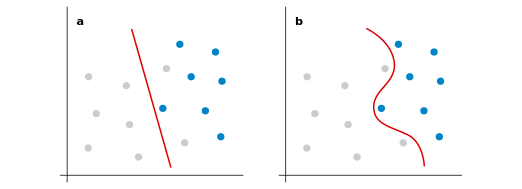
\includegraphics[width=\textwidth, keepaspectratio]{img/classifiers.pdf}
    	\caption{An example of two classifiers: A linear classifier (a) divides the data using a straight line but misclassifies two data points. A neural network (b) is able to learn a more complex decision boundary and separates the dataset without errors.}
    	\label{fig:classifiers}
	\end{figure}

Figure \ref{fig:classifiers} shows an example of two binary classifiers divide a simple dataset into two classes in 2D space. On the left-hand side is linear classifier dividing all points along a straight line. While this sort of classifier is very easy to train and understand it lacks the necessary foundation to divide more complex datasets. On the right-hand side is a neural network (more details in the next section) featuring a more complex, yet more accurate decision boundary. 

\subsection{Building Blocks of Deep Neural Networks}
Modern deep learning systems are constructed in a layer-wise fashion. Each layer does a non-linear computation to extract some feature and learns a representation of the input data before passing on its outputs to the next layer in the architecture. The term "deep" learning itself is not clearly defined but usually refers to having a at least two layered model. Typical state of the art systems have more than ten or more layers, some recent publication\cite{he2016deep} are even going as deep as 152 layers. While the total number of layers is be no means an indicator for an accurate and precise model it introduces the possibility to capture a larger and more generalized data representation.

\subsubsection{Fully Connected Layers}
\subsubsection{Convolutional Layers}

	\begin{figure}[]
  		\centering
    	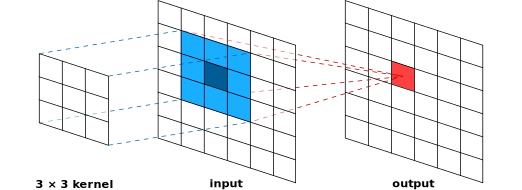
\includegraphics[width=\textwidth, keepaspectratio]{img/convolution.pdf}
    	\caption{A convolution of an image using a 3$\times$3 kernel. Each pixel in the output image is the weighted sum of nine pixels in the input image. The weights are defined by applied kernel and are learned by the model.}
    	\label{fig:convolution}
	\end{figure}

\subsubsection{Pooling Layers}

	\begin{figure}[]
  		\centering
    	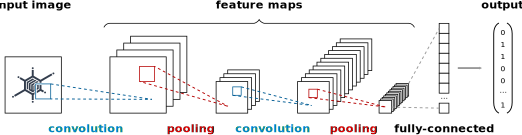
\includegraphics[width=\textwidth, keepaspectratio]{img/convnet.pdf}
    	\caption{A typical convolutional neural network architecture. An input image is fed through a series of convolutional and pooling layers. Each convolution extracts higher level features and increases number of feature maps. Each pooling layer subsamples the data, typically reducing the x and y dimension by half. A final fully connected layer serves as classifier able to predict an output value.}
    	\label{fig:convnet}
	\end{figure}

\subsubsection{Batch Normalization Layers?}
\subsubsection{Softmax Loss Function}

\subsection{Recurrent Neural Networks}
\subsubsection{Long Short Term Memory Networks}

\subsection{Hybrid Networks}
\label{sec:hybrid_networks}

	\begin{figure}[]
  		\centering
    	\includegraphics[width=\textwidth, keepaspectratio]{img/crnn.pdf}
    	\caption{Our proposed CRNN hybrid network architecture consists of two networks. A CNN transforms our input images into an intermediary representation of our audio frequencies. The 3D output of final convolutional layer of the CNN is sliced along the x-axis (time axis) into 2D time steps still containing all feature map information. The output of the final LSTM time step is fed into a fully connected layer for classification.}
    	\label{fig:crnn}
	\end{figure}
	
	\begin{figure}[]
  		\centering
    	\includegraphics[width=\textwidth, keepaspectratio]{img/crnn2.pdf}
    	\caption{An alternative approach for a hybrid CRNN network. Each single feature map of the final convolutional layer is fed to separate LSTM networks as a 2D input. Each LSTM interprets the vector entries along the x-axis as time steps and operates on thin slice of the data. The output of the final time step of each LSTM is concatenated into a single vector serving as the input to a fully connected classification layer.}
    	\label{fig:crnn}
	\end{figure}

    \begin{itemize}
        \item Convolutional Recurrent Neural Networks
        \item What is their purpose? Averaging over predictions / majority voting
    \end{itemize}

\subsection{Audio Representations}
\label{sec:audio_representations}
    \begin{itemize}
        \item MFCC
        \item Spectrogram (harmonics, formants)
        \item https://home.cc.umanitoba.ca/~robh/howto.html
        \item Waveform
        \item Mel-scale
        \item frequency --> phoneme --> word --> sentence --> language
    \end{itemize}
    \section{Related Work}
\label{sec:related_work}
In this chapter we lay out related work concerning neural network designs in general and hybrid networks which are specifically used for language identification. Additionally, we highlight related work on suitable input feature representations for machine learning on audio files. Furthermore, we present research on i-vector systems, the traditional approach to LID. Finally, we list related work on data augmentation. 

\subsection{Convolutional Neural Network Architectures}
With good results in the ImageNet Large Scale Visual Recognition Challenge (ILSVRC)\cite{ILSVRC15}, the \emph{AlexNet}\cite{krizhevsky2012imagenet}, \emph{VGGNet}\cite{simonyan2014very} and \emph{GoogLeNet}/\emph{Inception}\cite{szegedy2015going} have become the de-facto standard for neural network designs in the computer vision community.\\ 
Oxford university's visual geometry group published their deep neural network design which they called \emph{VGGNet}. Simonyan et al. proposed a convolutional neural network architecture with a depth of up to 16 or 19 weight layers.\cite{simonyan2014very, Chatfield14} They presented a thorough evaluation of increasing neural network depth using convolutional layers with 3$\times$3 kernel sizes and ReLU activations. Their system ended up winning the ILSVRC 2104 challenge.\\
Szegedy et al. reported on several iterations of Google's convolutional neural network architecture, called \emph{GoogLeNet} or \emph{Inception}.\cite{szegedy2015going, szegedy2016rethinking, szegedy2016inception} These deep and very deep convolutional neural networks repeatedly set the state-of-the-art record for minimal classification errors in the ImageNet competition. The presented network architectures present a number of advantages to previous CNN designs such as \emph{VGGNet}. Google introduced so-called inception modules or mini networks that aim to factorize convolutions with larger filter size in order to accelerate training time and reduce the amount of model parameters. The idea is to replace larger spatial filters (e.g 5$\times$5 and 7$\times$7) which are disproportionally expensive, in terms of computation with less expensive smaller inception modules with any loss of visual expressiveness. The inception modules are represented as a sequence of 3$\times$3 convolutions followed by a 1$\times$1 convolution. In case of replacing 5$\times$5 filters they were able to achieve a gain of 28\% in computational speed up. The resulting \emph{Inception-v2} and \emph{Inception-v3} networks consist of 42 layers and are trained using the RMSProp\cite{tieleman2012lecture} optimizer. Compared to the \emph{VGGNet}-style networks they feature a lower overall computational cost while offering higher accuracy on image vision tasks.

A second innovation introduced by the inception networks is the use of a technique called \emph{batch normalization}.\cite{ioffe2015batch} Training deep neural networks is particularly complicated through changes in the value distribution of each layer's input during training, as the parameters of the previous layer change. This slows down trainings by requiring lower learning rates and careful parameter initialization. Szegedy et al. refer to this phenomenon as \emph{internal covariate shift}. The proposed solution to this problem is to normalize the inputs of each mini batch for the following layer to unit vectors. This results in a number of benefits: Foremost they were able to drastically reduce the time need to converge their models. Batch normalization enabled them to use higher learning rates without running into the \emph{vanishing} or \emph{exploding gradient problem}. Furthermore, batch normalization acts as model regularizer positively affecting the generalization abilities of the network. In turn, this eliminates the need for dropout layers as regularizers. They conclude that simply by adding batch normalization to the convolutional layers of the inception network they were able to beat the state of the art of the ILSVRC challenge.

Shi et al. proposed an end-to-end trainable neural network for image-based sequence recognition and its application to scene text recognition.\cite{shi2016end} In their approach they used a hybrid neural network consisting of a convolutional part and a recurrent part for optical character recognition (OCR). The authors used convolutional layers as robust feature extractors for the input images and interpreted the resulting feature maps as a sequence of feature vectors. This sequence is fed into a LSTM network to capture the contextual information within the sequence. The whole CRNN was jointly trained with a \emph{connectionist temporal classification} (CTC) loss\cite{graves2006connectionist} to output a sequence of letters. They found a \emph{VGGNet}-based network architecture of seven convolutional layers with max pooling followed by a bidirectional LSTM to work best. The paper concludes that the use of \emph{batch normalization} greatly accelerated their training time. Additionally the authors employed 1$\times$2-sized rectangular pooling windows instead of conventional squared ones. This tweak yielded feature maps of larger width and hence longer sequences for the RNN.

\subsection{Spoken Language Processing Systems}
Much of the research around audio representations and spoken language processing is rooted in various related research communities: Music information retrieval (MIR), Automatic Speech Recognition (ASR) and Language Identification (LID). Alongside the rise in popularity of neural networks within the computer vision community we can witness their use for audio based tasks as well. Early LID system integrate and combine shallow neural networks within their i-vector systems (more details below).\cite{gonzalez2014automatic, han2013trap, matejka2014neural, richardson2015unified} These models usually feature no more than three layers and consist solely of classic neural networks or fully connected layers. While these systems neither benefit from the more efficient computation of CNNs nor the expressiveness of deeper systems they already were able to improve existing systems.

Song et al. reported the use of an end-to-end trainable, hybrid, convolutional recurrent neural network for automatic speech recognition (ASR).\cite{song2015end} They focussed on classifying a phoneme sequence of the input speech sample as part of their ASR system. Their proposed network consists of four convolutional layers, followed by two fully connected layers and is finalized by two LSTM layers. The network was jointly trained on the TIMIT dataset using CTC loss and mel-filter bank greyscale images as input. Given the short length of the individual phonemes they operates on audio snippets of 15-25 millisecond duration. Similarly to Shi et al. they apply rectangular pooling layers to obtain longer feature vector sequences.\cite{shi2016end} The reported results are competitive to traditional gaussian mixture models and hidden markov models for ASR tasks. 

Amodei et al. presented the Deep Speech 2 system for speech recognition. The system supports English and Mandarin Chinese as input languages.\cite{amodei2015deep} Their CRNN employed only three convolutional layers followed by seven bidirectional RNN or GRU layers. The model was trained end-to-end using CTC loss and a sequence of spectrograms of power-normalized audio as input. The model outputs a sequence of graphemes and uses a language model together with beam search to reconstruct words from the audio. The authors found both the LSTMs and GRU cells performed similarly well as the RNN layers. GRU cells, however, needed less computations and were less likely to diverge. For the CNN part the paper evaluated both the use of 1D time-only domain convolutions and 2D frequency-time domain convolutions. 2D Convolutions fared better especially with regard to noisy data.\\ 
Deep Speech 2 was trained with 12.000 hours of English Speech and 9.000 hours of Mandarin Chinese. Additionally, it used an increased dataset with augmented data boosting both their effective size of corpus as well as improving their noise robustness. For evaluation the authors also tested the system on accented speech and noisy speech read in coffee shops, streets, etc. In both scenarios the model's performance deteriorated.

\subsection{Methods of Input Data Representation}
There are many different types of audio representations used for spoken language processing. Many higher-level characteristics of sound relate to the energies in different frequency bands. This explains the utility of time-frequency representations of audio such as spectrograms, which are frequently used in literature.\cite{montavon2009deep, dieleman2013multiscale, lee2009unsupervised, wulfing2012unsupervised, henaff2011unsupervised} Alternatively, classical machine learning systems and i-vector systems usually rely on \emph{Mel-Frequency Cepstral Coeffiecient} (\emph{MFCC}) vectors\cite{richardson2015unified, dehak2011front, garcia2011analysis} or derivatives thereof such as perceptual linear prediction (PLP) coefficients\cite{gonzalez2014automatic}. Others have evaluated the use of raw waveform audio directly\cite{dieleman2014end, collobert2016wav2letter}.\\
Collobert et al. introduced Wav2Letter, an end-to-end convolutional neural network speech recognition.\cite{collobert2016wav2letter} They evaluated their system with three different input representations: Mel-Frequency Cepstral Coeffiecient (MFCC), spectrograms and raw waveform data. Here, a fully convolutional neural network performed best with MFCC vectors as input. Yet, power spectrograms still outperformed raw waveform inputs. This observation corresponded with Dieleman et al. who also noted that spectrograms are computationally cheaper given their already reduced and compacted representation.\cite{dieleman2014end} Raw audio, especially when sampled at a high rate of 44kHz, would increase the amount of striding width and window sizes of the employed convolutional layers.  
Deng et al. reported noticeably lower speech recognition errors using large-scale deep neural networks when using mel-scale filterbank spectrograms compared to MFCC features.\cite{deng2013recent}

\subsection{Language Identification Using i-vector Systems}
Prior to the neural-network-based deep learning systems mentioned above many researchers focussed on so-called identity vector (\emph{i-vector}) systems for spoken language processing tasks. Dehak et al. introduced i-vector systems for speaker verification tasks.\cite{dehak2011front} I-vectors are a representation obtained by mapping a sequence of frames of a given utterance into a low-dimensional vector space based on a factor analysis technique. This is referred to as the total variability space.  Typically such a system is designed as follows. First, a feature extractor is used to turn an audio file into a 20 dimensional mel-frequency cepstral coefficient (MFCC) vector or a 56 dimensional shifted delta cepstral (SDC) vector. These are then used to train a unified background model (UBM), a speaker and language-independent Gaussian mixture model (GMM). Different speakers have different subspaces within this universal acoustical cluster inside the UBM. The trained, high dimensional GMM supervector is decomposed into its individual components to obtain individual speaker and language dependent characteristics. Matrix decomposition methods such as principal component analysis (PCA) can be used for the decomposition step. For this, the i-vector is whitened by subtracting a global mean, scaled by the inverse square root of a global covariance matrix, and then normalized to unit length.\cite{garcia2011analysis} Typically the i-vector is a compact representation of 400-600 dimensions. Finally, a score between the model and the i-vector of a test sample is computed. The simplest scoring measure is the cosine distance between the embedded i-vectors of languages.

Other research experimented with linear discriminant analysis (LDA) and neighborhood component analysis (NCA) for dimensionality reduction of the UBM.\cite{dehak2011front} Sizov et al. reported the use of probabilistic linear discriminant analysis (PLDA) for this job.\cite{sizov2016discriminating}\\
While many systems share i-vectors as the input to a classifier the actual type of classification algorithm varies widely. For language identification Dehak et al. used support vector machines (SVM) with cosine kernels.\cite{dehak2011front} Others employed logistic regression\cite{martinez2011language} or used a simple three layer neural network\cite{plchot2016bat}. Gonzalez et al. outperformed all previous attempts by using a four layer deep neural network.\cite{gonzalez2015frame} Gelly et al. presented the use of bidirectional LSTMs with i-vectors.\cite{gelly2016language} Other submissions to NIST LRE 2015 challenge\cite{lre2015} include many further research approaches with i-vector systems including the use of stacked bottleneck features, bayesian unit discovery and model fusions.\cite{lee20162015, torres2008mitll, ng2016sheffield} This feature engineering around i-vectors results in more complex systems with an increasing number of processing and computational steps in their pipeline. Zazo et al. did a comparison analysis between i-vector systems and LSTM networks and found the latter to perform better in some settings and to be on par in others.\cite{zazo2016evaluation} They also note, that the LSTM network used about 85\% less parameters than a classical i-vector system while achieving robust and comparable results in several challenging scenarios.

\subsection{Methods For Data Augmentation}
Last, we present related work to data \emph{augmentation}. To overcome insufficient variety in a dataset or to extend its size, researchers supplement their data with artificially created or augmented files. This approach not only boosts the overall dataset size but helps to improve a model's ability to generalize by learning from more diverse samples. For computer vision tasks, Szegedy et al. proposed to scale, translate, rotate, deform and mirror the input images.\cite{szegedy2015going} All these modifications are, however, some form of image manipulation. For audio data there are alternative approaches, too. Similarly to image scaling, one can change the playback speed of audio data by changing the sampling rate. There are two downsides to this approach, though. First, randomized time stretching changes the audio pitch. Speeding up audio results on speech recordings of unnaturally high pitched voices. Second, manipulation the time domain alters the length of pauses between words and frequency activations. Such extreme modifications could render the augmented data incompatible to the original dataset. Ko et al. recommendeD changing the speed of the audio signal to no less than 90\% and no more than 110\% of original signal speed.\cite{ko2015audio} The largest benefit of this augmentation method is its simplicity and low implementation cost.

Amodei et al. noted that the introduction of background noise into their data helped to improve speech recognition robustness for noisy speech samples in general.\cite{amodei2015deep} They augmented about 40\% of their dataset with randomly selected audio clips. We will explore this approach in our system, too. Results of this are documented in a later chapter. Cui et al. proposed the use of stochastic feature mapping in order to transfer one speaker's speech features to another.\cite{cui2015data} Their approach attempted to apply voice conversion for languages like Bengali and Assam, both of which are spoken only by small communities and hence needed to increase the limited amount of available digital speech recordings.\\ 
Jaitly et al.\cite{jaitly2013vocal} introduced what they called \emph{Vocal tract length perturbation} (VTLP) to improve speech recognition systems. Inspired by previous work on Vocal Tract Length Normalization \cite{eide1996parametric}, which removes speaker-to-speaker variations using normalization methods, they warped the frequency of each utterance by a random factor. Using VTLP they were able to decrease the recognition error on their evaluation dataset.

       
    \section{Datasets}
	In this section we will explain the structure of our datasets, how we obtained them and what preprocessing steps are needed to extract our features.

	Recent breakthroughs in deep learning were fueled by the availability of large-scale, well-annotated, public datasets, e.g. ImageNet \cite{ILSVRC15}. Within the language identification community the TIMIT corpus of read speech \cite{garofolo1993darpa} has long been the default test set. TIMIT contains a total of 5.4 hours, consisting of 10 sentences spoken by each of 630 speakers from 8 major dialect regions of the United States recorded at 16kHz. Given the short span of each individual sound clip, the overall corpus duration and limitation to one language it was necessary to obtain our data from somewhere else. 
  
  	This thesis uses two primary datasets collected and processed by us. On the one hand we use speeches and statements from the European Parliament and on the other hand we rely on reports from news broadcasts sourced from YouTube.

\subsection{Language Selection}  

\subsection{EU Speech Repository}

	The EU Speech Repository is a collection of video ressources for interpretation students provided for free by the European Commission. The dataset is made up from debate of the European Parliament, commitee press conferences, interviews and tailor-made training material from EU interpretors. All audio clips are recorded in the speaker's native language and feature only one speaker.
	
		With 131 hours of speech data it is the smaller of the two datasets. We obtained material in four languages: English, German, French, and Spanish

\subsection{YouTube News Collection}

	Following the example of Montavon \cite{montavon2009deep} we looked for large, public sources of speech audio. We first experimented with podcasts and radio stations, both of which are unsuited for the job. Podcasts usually feature only one speaker and radio contains a lot of noise in the form of music. From these initial insights we noticed that news broadcasts provided high quality speech audio data. To source a large variety of languages and gather enough hours of speech audio we sourced the majority of our data from YouTube. 
	
	For each target language we manually select one or more YouTube channels of respected news outlets. E.g. for English we used the BBC and CNN to gather a variety of different accents. For a full list of channels refer to table \ref{tab:channels}. All channels were chosen regardless of their content, their political views or journalistic agenda.
	
	\begin{table}[]
	\centering
	\begin{tabular}{@{}ll@{}}
	\toprule
	YouTube Channel Name  & Language \\ \midrule
	CNN                   & English \\
	BBCNews               & English \\
	VOAvideo              & English \\
	DeutscheWelle         & German \\
	Euronewsde            & German \\
	N24de                 & German \\
	France24              & French \\
	Antena3noticias       & Spanish \\
	RTVE                  & Spanish \\
	VOAChina              & Mandarin Chinese  \\
	Russia24TV            & Russian \\
	RTrussian             & Russian \\ \bottomrule
	\end{tabular}
	\label{tab:channels}
	\caption{YouTube Channel names and their corresponding language}
	\end{table}

  	
  	Audio obtained from news coverage has many desired properties. The data is of high recording quality and hundreds of hours recording is available online. News anchors are trained to speak loud and clear, while still talking at a normal speed. News shows often feature guests or correspondents so we get a variety of speakers, which converse in a ordinary fashion with each other unlike speech audio obtained from reading texts aloud. Lastly, news shows feature all the noise one would expect from a real world situation: music jingles, non-speech audio from video clips and transitions between reports. In essence we believe that speech data source from news broadcast represent an accurate, real-world sample for speech audio.
  	
  	In contrast to the EU Speech Repository this dataset consists 1024 hours of audio data for the same four languages: English, German, French and Spanish. We also gathered an extended language set adding Mandarin Chinese and Russian to the dataset. The extended set is only used for the evaluation of the model extensibility as outlined in section \ref{sec:extensibility}. Table \ref{tab:dataset_comparison} provides a complete comparison between the datasets.
  	

	\begin{table}[]
	\centering
	\begin{tabular}{@{}llll@{}}
	\toprule
	Feature               & EU Speech Repository & YouTube News & YouTube News Extended \\ 
	\midrule
	\# Languages   		  & 4                    & 4            & 6                     \\
	Total audio duration  & 4                    & 4            & 6                     \\
	Average clip duration & 4                    & 4            & 6                     \\
	Sample Rate           & 4                    & 4            & 6                     \\ 
	\# Training Samples   & 4                    & 4            & 6                     \\ 
	\bottomrule
	\end{tabular}
	\label{tab:dataset_comparison}
	\caption{Comparison of the EU Speech and YouTube News dataset}
	\end{table}
	
	
\subsection{Preprocessing}

- train / test split
- number of training samples
- sample creation / preprocessing



    \section{Implementation}
This section will outline the employed software and hardware resources of the system, explain the data preprocessing, and describe the model architecture of our neural networks in detail.

\subsection{Software}
\label{sec:software}


	The language identification system is implemented in Python. We used the open source deep learning framework Keras\cite{chollet2015keras} with the TensorFlow\cite{abadi2016tensorflow} backend for training our neural networks. Keras provides us with a set of higher level machine learning primitives such as convolutional layers and optimizing algorithms without abstracting too much away. Internally it builds on Google's open source numerical operation library TensorFlow which is optimized to quickly compute large multidimensional data on GPUs.
		
	 
	From a high level perspective, our system was designed in three parts. 
	
	\begin{description}
		\item[The preprocessor] Its job is to download, extract, and convert the data. The preprocessor clips the audio tracks for raw video footage and converts them into WAV files before ultimately converting the data into PNG images for the training. Details can be found in section \ref{sec:data_processing}.
		\item[The trainer]
		\item[The evaluator] 
	\end{description}
	

\subsection{Data Preprocessing}
\label{sec:data_processing}
All audio files have to be preprocessed before feeding them to the neural network. As a first step all files are encoded as uncompressed, lossless Waveform Audio File Format\footnote{\url{http://www.microsoft.com/whdc/device/audio/multichaud.mspx}, accessed 23.02.2017}, WAVE, commonly know by its file extension *.wav. This conversion has two advantages: A lossless data codec allows for future audio manipulations with any quality loss and makes the data easily readable by third party programs and library such as SciPy\footnote{\url{https://www.scipy.org/}, accessed 23.02.2017}. 

	Since our CNN does not operate on raw waveform audio signals we transfer it into the image domain. As introduced in section \ref{sec:audio_representations} we used a spectrogram representation of the audio file for model training. The spectrograms were generated using the open source command line tool SoX\footnote{\url{http://sox.sourceforge.net/}, accessed 23.02.2017}. Spectrograms are generated using a Hann window and 129 frequency bins along the frequency-axis (y-axis). The time-axis (x-axis) is rendered at 25 pixel per second. Each audio sequence is clipped into non-overlapping ten second segments. The  final segment is discarded to avoid segments shorter than the required ten seconds. We decided against filtering silent section within the audio segment to keep the natural pauses between words and not disturb the regular speech rhythm. Frequency intensities are mapped to a gray scale. The resulting greyscale images are saved as lossless PNG files and are 500 pixel in width and 129 pixel in height. Appendix \ref{sec:appendix_a} includes the complete listing \ref{lst:spectrograms} for generating spectrogram images with SoX.
	
	As can be seen in figure \ref{fig:spectrogram} the spectrograms feature very apparent bright ripple-like pattern. Each of these represents a strong activation of a certain frequency over time. Several frequency activations can be active at once constituting a particular phoneme or sound. A sequence of these phonemes forms words and is only interrupted by short speech pauses. It is our aim to learn the characteristic and unique composition of these frequency activation for every language in our classifier. 

	
	\begin{figure}[h]
  		\centering
    	\includegraphics[width=\textwidth,keepaspectratio]{img/spectrogram.png}
    	\caption{A spectrogram generated from a ten second German audio clip  using SoX. Notice the bright ripple-like patterns. These frequency activations serve as the main features for the classifier.}
    	\label{fig:spectrogram}
	\end{figure}
	
    \begin{itemize}
        \item Spectrogram Generation
        \item Data Segmentation
        \item (Augmentation)
        \item train / test split
		\item number of training samples
    \end{itemize}

\subsection{CNN Architecture}
\label{sec:cnn_architecture}


    \begin{itemize}
        \item Layer Table
        \item Transfer Learning / Fine-tuning
        \item Variations
    \end{itemize}
    
    \begin{table}[h]
  \centering
  \begin{tabularx}{\textwidth}{Xllll}
  \toprule
  Layer Type                       & input maps  & output maps & kernel & stride  \\ \midrule
  \mbox{Convolution with} \mbox{Batch Normalization}  & 1           & 16     & 7x7    & 1       \\ 
  Max Pooling                           & 16          & 16     & 2x2    & 2       \\ 
  Convolution with Batch Normalization  & 16          & 32     & 5x5    & 1       \\ 
  Max Pooling                           & 32          & 32     & 2x2    & 2       \\ 
  Convolution with Batch Normalization  & 32          & 64     & 3x3    & 1       \\ 
  Max Pooling                           & 64          & 64     & 2x2    & 2       \\ 
  Convolution with Batch Normalization  & 64          & 128    & 3x3    & 1       \\ 
  Max Pooling                           & 128         & 128    & 2x2    & 2       \\ 
  Convolution with Batch Normalization  & 128         & 256    & 3x3    & 1       \\ 
  Max Pooling                           & 256         & 256    & 2x2    & 2       \\ 
  Dropout                               &             &        &        &         \\ 
  Fully Connected                       & ???         & 1024   &        &         \\ 
  Fully Connected                       & 1024        & 4      &        &        \\ 
  \bottomrule
  \end{tabularx}
  \caption{The layer architecture for the convolutional neural network CNN\_A.}
  \label{tab:layers_CNN_A}
  \end{table}
    
    

\subsection{CRNN Architecture}

    \begin{itemize}
        \item Layer Table
        \item Architecture Image
        \item Conv Features to time steps
        \item Transfer Learning / Fine-tuning
        \item 
    \end{itemize}

    \section{Evaluation}

\subsection{Setup}
\subsubsection{Data}
\subsubsection{Training of the Neural Network Model}
\subsubsection{Validation of the Training Process}

\subsection{Evaluation Metrics}
\subsubsection{Application Dependent Evaluation}
\begin{itemize}
    \item F1
    \item Accuracy, error rate
    \item Precision, Recall
\end{itemize}
\subsubsection{Application Independent Evaluation}
\begin{itemize}
    \item Equal Error Rate
    \item $$c_avg$$
\end{itemize}


\subsubsection{Discussion and Comparison}
\subsubsection{Experiments}

    \section{Demo Application}
- web service
- python, react, flask
- image
- default examples




    \section{Conclusion and Future Work}
\label{sec:summary}
This last chapter presents high-level insights and finally comments on
future work and prospects concerning the discussed topics.
It further outlines the contribution of this thesis and concludes the work done
in the research field.

\subsection{Future Work}
The overall trend within the deep learning community over the past few years has been to increase the network depth by adding more and more layers. Supporting this development, however, is becoming increasingly more difficult. Very deep networks are harder to train and require ever more computing time. One way to gain higher accuracy scores is to change the design and architecture of the network. He et al. recently proposed the technique of deep residual learning\cite{he2016deep} to tackle these challenges. In their network architecture they introduce small building blocks of two convolutional layers in which the second layer receives the original input of the first layer in addition to the output of its predecessor~\cite{he2016deep}. Using this approach, they were able to train \emph{ResNet} with 152 layers and bested the previous state of the art in the ILSVRC 2015 challenge. Similarly, Szegedy et al. introduced the latest iteration of their Inception networks using these residual connections\cite{szegedy2016inception} as well.

For future work, we think that using deep residual neural network for the convolutional part of our architecture holds much promise. In this thesis we were able to measure our best results using the previously state-of-the-art \emph{Inception-v3} network for computer vision tasks. In the future we believe that using \emph{Inception-v3} or the ResNet architecture should improve our results even further and perhaps add more robustness to noise as well.

As part of our training process, we pretrained our convolutional neural networks before assembling them to the complete CRNN. The complete CRNN then reused the learned weights of the convolutional layers and finetuned them by further, joint training with the LSTM part. This \emph{transfer learning} approach is fairly simple, yet effective. Unfortunately, parallel to finetuning the network on the new data it starts to forget previously learned features. This is referred to as catastrophic forgetting. Rusu et al. introduced \emph{Progressive Neural Networks}~\cite{rusu2016progressive} as a novel approach to \emph{transfer training}. This technique leverages prior knowledge via so called lateral connections to previously learned features. For future work, we think it is worthwhile to evaluate whether this approach could be helpful in improving our transfer learning steps.

We formulated our research problem as a classification problem for language identification. The limitation of this, however, is that our models are only able to accurately predict languages that have been part of the training corpus. In other words, we are unable to identify any language unknown to the system. An interesting, yet slightly different research field, is metric learning. This approach is able to measure a difference or a score between its classes. So for example with metric learning, a sample would receive a score whether it was closer related to German or English. The advantage of this approach is that the system is no longer limited to only the training languages. For unknown languages one could still assess, whether a language is more similar to one then another. Conversely, this also allows to judge how different an input is to any language know to the system, something that is not possible with our approach.

In this thesis we evaluated our networks on six different input languages. In the future our system could be extended to cover even more languages. In our work we did not evaluate the effectiveness of the presented approach on similar tasks such as dialect identification. Future work could evaluate the accuracy of our approach on the fine grained differences between dialects and accents of a language.

Throughout this work we evaluated our models' robustness to white noise and background music noise. We also tried evaluating our models on songs but found the performance to be inadequate for our needs. In our case the biggest problem with songs was the fact that the speech frequencies are completely masked by the frequencies of the different instruments. Future work could focus on language identification for songs and music.

Our approach relies on extracting and classifying a sequence of intermediate languages representation created from spectrogram image inputs. Within the automatic speech recognition (ASR) community there is related work that extracts and classifies a sequence of phonemes~\cite{song2015end}. Instead of matching these phoneme sequences to words one could use these to classify a target language. This is an alternative approach to the one presented in this thesis and could be used to compare the effectiveness and robustness of the two methods. Another interesting idea was introduce by Google's \emph{Wavenet}~\cite{van2016wavenet}. Utilizing dilated convolutions for speech recognition they were able to capture a longer receptive field while being much cheaper to compute than LSTMs. Further, \emph{Wavenet} operates on raw audio signals forgoing the need for spectrogram features.  Even though they evaluated \emph{Wavenet} for automatic speech recognition, it could likely be adopted to language identification as well. 

\subsection{Conclusion}
In this thesis we presented several neural network architectures aimed at the task of solving the language identification problem. We employed CNNs and CRNNs to infer the language of a given audio sample directly from its spectrogram representation. 

We proposed three hypotheses and conducted experiments to verify their validity. We confirmed that, first convolutional neural networks are an effective, high-accuracy solution for language identification tasks. Second, spectrogram images are a suitable input representation for learning audio features. Third, convolutional recurrent neural networks consistently improve the classification accuracy throughout all experiments compared to a plain, CNN-based approach.

We present and discuss the availability and suitability of various datasets for LID. For our research we compiled and processed more than a thousand hours of speech data from public sources. On the one hand, this thesis gathered speeches and press conferences from the European Parliament. On the other hand, we collected audio from news broadcasts hosted on YouTube.

To judge the effectiveness and validity of our research in several scenarios, we augmented our test dataset with additional white noise, crackling noise, and background music and tested the robustness of our neural networks. We report a decrease in recognition accuracy under these noisy situations.

In this work, we explored different neural network architectures and comment on our setup of hyperparameters. Our best performing CRNN model is based the Inception-v3 architecture and was able to achieve an accuracy and F1~score of~\num{0.96} and~\num{0.96}, respectively.

Initially, we trained and evaluated our models on four languages---English, German, French, and Spanish. We were content to find that the approach presented in this thesis could be transferred to other languages as well. During our experiments we added Mandarin Chinese and Russian. The frequency features learned by our system are, indeed, language-independent and we were able to expand our system to these two new languages without any large modifications.

This thesis presents a recent approach to solve the language identification task with deep neural networks. Further research needs to be deducted to improve the robustness against noise and discover new kinds of layers and architectures to support even higher accuracies in this field. 

    \begin{appendices}
\section{Audio manipulation with SoX}
\label{sec:appendix_a}

        \begin{lstlisting}[caption=Adding white noise to an audio file]
    scale_factor1=0.94; 
    scale_factor2=0.05;
     
    sox -m \
        -v $(echo "$(sox input.wav -n stat -v 2>&1) * ${scale_factor1}" | bc -l)  input.wav \
        -v ${scale_factor2} <(sox input.wav -p synth whitenoise) \
        -b 16 output.wav
   \end{lstlisting}
   
\section{Background Music Evaluation Sources}

	\begin{table}[h!]
	\centering
	\begin{tabularx}{\textwidth}{ll}
\toprule
English  & \\ \midrule
HipHop  & \url{https://www.youtube.com/watch?v=uelHwf8o7_U&list=RDQMENRLh0JQHf4} \\ 
Pop     & \url{https://www.youtube.com/watch?v=hT_nvWreIhg&list=RDQMxXC2APeBvGc} \\   
\toprule
German  & \\ \midrule
HipHop  & \url{https://www.youtube.com/watch?v=y8pcVDN8vWQ&list=RDQMSi8P9Y1QpqM} \\ 
Pop     & \url{https://www.youtube.com/watch?v=kiMG_JV2gbo&list=RDQM10mSCd8-mJo} \\   
\toprule
French  & \\ \midrule
HipHop  & \url{https://www.youtube.com/watch?v=-n8kGW16RYs&list=RDQMUV6pew7j0sI} \\ 
Pop     & \url{https://www.youtube.com/watch?v=yleB8fUXudw&list=RDQMCawvWO0Heyc} \\   
\toprule
Spanish  & \\ \midrule
HipHop  & \url{https://www.youtube.com/watch?v=CUYrEiymUMY&list=RDQMYSngtE3m2uY} \\ 
Pop     & \url{https://www.youtube.com/watch?v=tIpzfs5tBJU&list=RDQMJhi12p5mKDc} \\   
 	\bottomrule
	\end{tabularx}
	\caption{}
	\label{tab:audio_sources}
	\end{table}

\end{appendices}

    % Inhaltsverzeichnis
    \clearpage % auf neuer Seite
    \bibliography{referenzen}

\end{document}
